% Created 2018-11-17 sáb 14:11
% Intended LaTeX compiler: pdflatex
\documentclass[xcolor={usenames,svgnames,dvipsnames}]{beamer}
\usepackage[utf8]{inputenc}
\usepackage[T1]{fontenc}
\usepackage{graphicx}
\usepackage{grffile}
\usepackage{longtable}
\usepackage{wrapfig}
\usepackage{rotating}
\usepackage[normalem]{ulem}
\usepackage{amsmath}
\usepackage{textcomp}
\usepackage{amssymb}
\usepackage{capt-of}
\usepackage{hyperref}
\usepackage{color}
\usepackage{listings}
\usepackage{mathpazo}
\usepackage{gensymb}
\usepackage{amsmath}
\usepackage{chemarr}%flechas para reacciones químicas (SFER.tex)
\bibliographystyle{plain}
\AtBeginSubsection[]{\begin{frame}[plain]\tableofcontents[currentsubsection,sectionstyle=show/shaded,subsectionstyle=show/shaded/hide]\end{frame}}
\AtBeginSection[]{\begin{frame}[plain]\tableofcontents[currentsection,hideallsubsections]\end{frame}}
\usepackage[emulate=units]{siunitx}
\sisetup{fraction=nice, decimalsymbol=comma, retain-unity-mantissa = false}
\newunit{\wattpeak}{Wp}
\newunit{\watthour}{Wh}
\newunit{\amperehour}{Ah}
\usepackage{steinmetz}
\hypersetup{colorlinks=true, linkcolor=Blue, urlcolor=Blue}
\renewcommand{\thefootnote}{\fnsymbol{footnote}}
\beamertemplatenavigationsymbolsempty
\setbeamertemplate{footline}[frame number]
\setbeamercolor{alerted text}{fg=blue!50!black} \setbeamerfont{alerted text}{series=\bfseries}
\usetheme[hideothersubsections]{Goettingen}
\usecolortheme{rose}
\usefonttheme{serif}
\author{Oscar Perpiñán Lamigueiro}
\date{\url{http://oscarperpinan.github.io}}
\title{Bases de Datos de Radiación Solar}
\subtitle{Energía Solar Fotovoltaica}
\hypersetup{
 pdfauthor={Oscar Perpiñán Lamigueiro},
 pdftitle={Bases de Datos de Radiación Solar},
 pdfkeywords={},
 pdfsubject={},
 pdfcreator={Emacs 25.2.2 (Org mode 9.1.13)}, 
 pdflang={Spanish}}
\begin{document}

\maketitle

\section{Bases de Datos}
\label{sec:orgd908399}
\subsection{Introducción}
\label{sec:org23147ce}

\begin{frame}[label={sec:org58d0ea5}]{Variabilidad Temporal y Espacial}
\begin{itemize}
\item La irradiancia solar extraterrestre depende de la latitud y el instante temporal (\emph{proceso determinista}).
\item La irradiancia solar incidente en la superficie terrestre es resultado de la interacción con la atmósfera cambiante: \alert{variabilidad temporal y espacial} (\emph{proceso estocástico}).
\end{itemize}
\end{frame}

\begin{frame}[label={sec:orga24d126}]{Variabilidad Temporal}
Variabilidad de la irradiación diaria, mensual y anual durante el período comprendido entre 2001-2008 en Carmona, Sevilla
\begin{center}
\includegraphics[width=.9\linewidth]{../figs/VariabilidadRadiacionDiario.pdf}
\end{center}

\nocite{Perpinan2009}
\end{frame}

\begin{frame}[label={sec:org0582560}]{Variabilidad Temporal}
\[
\sigma_{\overline{G}}=\frac{\sigma_{G}}{\sqrt{N}}
\]

\begin{itemize}
\item Predicción para un (día, mes, año) \alert{determinado}: 

\begin{itemize}
\item Intervalo de confianza del 95\% acotado por \(1.96\cdot\sigma_{G}\)
\end{itemize}

\item Predicción para un (día, mes, año) \alert{promedio (durante N años)}: 

\begin{itemize}
\item Intervalo de confianza del 95\% acotado por \(1.96\cdot\sigma_{\overline{G}}\)
\end{itemize}
\end{itemize}
\end{frame}

\begin{frame}[label={sec:orgf984091}]{Variabilidad Espacial}
\begin{center}
\includegraphics[width=0.9\textwidth]{../figs/SpatialVariability.jpg}
\end{center}

\[
COV = 1/G_p \sqrt{\frac{\sum_1^{n}(G_p^2 - G_i^2)}{n}}
\]

\nocite{Gueymard.Wilcox2011a}
\end{frame}

\begin{frame}[label={sec:orgaf0e12e}]{Variabilidad Espacial}
\begin{center}
\begin{center}
\includegraphics[height=0.9\textheight]{../figs/SpatialVariability_Annual.jpg}
\end{center}
\end{center}
\end{frame}

\begin{frame}[label={sec:org771d867}]{Estimación a partir de Medidas}
\begin{itemize}
\item Para estimar la radiación incidente es necesario contar con:
\begin{itemize}
\item \alert{Medidas cercanas} (variabilidad espacial): distancia no superior a 10 km.
\item \alert{Series temporales} largas (variabilidad temporal): 10 años.
\end{itemize}
\end{itemize}
\end{frame}

\begin{frame}[label={sec:org82b4e09}]{Fuentes de datos}
\begin{itemize}
\item \alert{Estaciones meteorológicas}
\begin{itemize}
\item Series largas y con tiempos de muestreo altos.
\item Baja resolución espacial (medidas puntuales)
\item Precisión en caso de medida directa.
\item Tipos: 
\begin{itemize}
\item Con medidor de radiación
\item Sin medidor de radiación (modelos empíricos).
\end{itemize}
\end{itemize}
\end{itemize}

\pause

\begin{itemize}
\item \alert{Imágenes de satélite}

\begin{itemize}
\item Tiempos de muestreo bajos (mejorando)

\item Resolución espacial alta

\item Error debido a la estimación.
\end{itemize}
\end{itemize}

\pause 

\begin{itemize}
\item \alert{Híbrido}

\begin{itemize}
\item Medidas terrestres combinadas con imágenes de satélite
\end{itemize}
\end{itemize}
\end{frame}

\subsection{Estaciones Meteorológicas}
\label{sec:org363c007}
\begin{frame}[label={sec:org6a4889c}]{Estaciones Meteorológicas: medida directa}
\begin{block}{La medida directa de radiación solar se realiza con un piranómetro.}
\end{block}
\begin{columns}
\begin{column}{0.4\columnwidth}
\begin{center}
\begin{center}
\includegraphics[width=0.8\textwidth]{../figs/piranometro.jpg}
\end{center}
\end{center}
\end{column}
\begin{column}{0.6\columnwidth}
\begin{itemize}
\item Pila termoeléctrica (termopares con barniz negro)
\item Alojamiento con dos hemiesferas de cristal.
\item Flujo de calor por radiación provoca tensión eléctrica en termopila.
\end{itemize}
\end{column}
\end{columns}
\end{frame}

\begin{frame}[label={sec:org7ab4726}]{Estaciones Meteorológicas: medida directa}
\begin{block}{La medida directa de radiación solar se realiza con un piranómetro.}
\end{block}
\begin{columns}
\begin{column}{0.4\columnwidth}
\begin{center}
\begin{center}
\includegraphics[width=0.8\textwidth]{../figs/piranometro.jpg}
\end{center}
\end{center}
\end{column}
\begin{column}{0.6\columnwidth}
\begin{itemize}
\item Respuesta espectral plana para radiación visible.
\item Respuesta perfecta al coseno del ángulo de incidencia (pérdidas por reflexión).
\end{itemize}
\end{column}
\end{columns}
\end{frame}


\begin{frame}[label={sec:org400bca1}]{Estaciones Meteorológicas: medida directa}
\begin{block}{La medida directa de radiación solar se realiza con un piranómetro.}
\begin{itemize}
\item Requiere mantenimiento y calibración frecuente.
\end{itemize}
\end{block}

\begin{block}{La red de estaciones que miden directamente radiación es escasa para estimaciones precisas en regiones grandes}
\begin{itemize}
\item La proporción de estaciones con piranómetros es baja respecto a
las que miden temperatura ambiente y precipitación (1:500).
\end{itemize}
\end{block}
\end{frame}

\subsection{Estaciones Meteorológicas: modelos empíricos}
\label{sec:orga4f7667}
\begin{frame}[label={sec:org6ac4044}]{Frente a la baja densidad de estaciones con medida directa de radiación se emplean modelos empíricos}
\begin{itemize}
\item Relaciones entre radiación y otras variables
\begin{itemize}
\item Horas de brillo (\emph{sunshine duration})
\item Cobertura nubosa
\item Temperatura ambiente
\item Precipitación
\item Humedad
\item \ldots{}
\end{itemize}
\item Los coeficientes de los modelos sólo se pueden ajustar en estaciones
con medidas de radiación.
\item Los coeficientes dependen del lugar de ajuste, pero se pueden
interpolar para otras localizaciones.
\end{itemize}
\end{frame}

\begin{frame}[label={sec:orgd3d9701}]{Estaciones Meteorológicas: modelos empíricos}
\begin{itemize}
\item Radiación y Horas de Brillo (Angstrom y Prescott)
\end{itemize}

\[
\frac{G(0)}{B_o(0)} = a_1 + b_1 \frac{S}{S_o}
\]

\begin{itemize}
\item Problema: poca disponibilidad de datos
\end{itemize}
\end{frame}

\begin{frame}[label={sec:org306014f}]{Estaciones Meteorológicas: modelos empíricos}
\begin{itemize}
\item Radiación y Temperatura (Bristow y Campbell)
\end{itemize}
\[
G(0) = a \left(1 - \exp(-b \Delta T^c)\right) \cdot B_o(0)
\]

\begin{itemize}
\item Variaciones con más variables: Lluvia (si/no), rango antes y después, velocidad viento, humedad relativa.
\end{itemize}

\[
  G(0) = a \left(1 - \exp(-b \Delta T^c)\right) \cdot B_o(0) \cdot \left(1 +
    \sum_1^n p_j \cdot v_j \right) + p_{n+1}
\]

\nocite{Antonanzas-Torres.Sanz-Garcia.ea2013}
\end{frame}

\subsection{Imágenes de Satélite}
\label{sec:orgcfa81a4}

\begin{frame}[label={sec:org230edc6}]{Fundamentos}
\begin{itemize}
\item Los satélites meteorológicos están equipados con \alert{radiómetros}
(sensores de radiación electromagnética a diferentes frecuencias)
que captan \alert{radiación emitida por la Tierra}.

\item La radiación emitida por la Tierra depende de la \alert{reflexión del
suelo}, y la \alert{geometría y composición de la atmósfera}.

\item Diferentes fenómenos físicos se detectan en \alert{bandas de frecuencias}
distintas (canales).

\item Existen diversos procedimientos para \alert{estimar radiación solar} en
superficie a partir de la información de los diferentes canales del
radiómetro.
\end{itemize}
\end{frame}

\begin{frame}[label={sec:org5bfba3e}]{Satelites Geoestacionarios Europeos: Meteosat}
\begin{itemize}
\item \alert{MFG}: Meteosat First Generation (7 satélites)
\begin{itemize}
\item Equipados con el radiómetro MVIRI (Meteosat Visible and Infrared Imager).
\item Tres canales: visible, infrarrojo, vapor de agua.
\end{itemize}
\item \alert{MSG}: Meteosat Second Generation (3 satélites)
\begin{itemize}
\item Equipados con dos radiómetros:
\begin{itemize}
\item \alert{SEVIRI} (Spinning Enhanced Visible and InfraRed Imager): 12 canales
\item GERB (Geostationary Earth Radiation Budget): infrarrojo visible.
\end{itemize}
\end{itemize}
\end{itemize}

\begin{center}
\begin{center}
\includegraphics[height=0.3\textwidth]{../figs/Tierra_MSG.jpg}
\end{center}
\end{center}
\end{frame}


\begin{frame}[label={sec:org1d5670e}]{Procedimientos: Heliosat-2}
\begin{block}{Pasos}
\begin{itemize}
\item Establecer \alert{albedo de referencia} (\emph{suelo}).
\item Estimar \alert{índice de cobertura nubosa}.
\item Estimar radiación en superficie a partir de cobertura nubosa y \alert{modelo de cielo claro}.
\end{itemize}
\end{block}

\begin{block}{}
\begin{itemize}
\item Empleado para base HelioClim
\item Usan datos de MVIRI
\item Accesible via SoDa: \url{http://www.soda-is.com/heliosat/index.html}
\end{itemize}

\nocite{Rigollier.Lefevre.ea2004}
\end{block}
\end{frame}

\begin{frame}[label={sec:org4f16fa8}]{Procedimientos: CM SAF}
\begin{itemize}
\item \alert{Fundamento}:
\begin{itemize}
\item Se emplea un \alert{Radiative Transfer Model (RTM)}, libRadtran, para
generar una matriz de estados (\alert{Look-up table, LUT}) relaciona la
transmitancia atmosférica y el albedo de la atmósfera para
variedad de estados.
\item La irradiancia en superficie se estima multiplicando la
irradiancia extra-atmosférica por la \alert{transmitancia atmosférica
determinada interpolando en la LUT}.
\end{itemize}
\end{itemize}

\pause

\begin{itemize}
\item \alert{Dos LUTs}: cielo nuboso, cielo claro.
\begin{itemize}
\item \alert{Cielo nuboso}:
\begin{itemize}
\item Estimación de albedo y estado atmosférico a partir de imágenes.
\item Estimación de transmitancia interpolando en LUT para cielo nuboso.
\end{itemize}
\item \alert{Cielo claro}:
\begin{itemize}
\item Estimación de transmitancia interpolando en LUT para cielo claro \alert{sin estimación previa} de albedo.
\end{itemize}
\end{itemize}
\end{itemize}

\pause

\begin{itemize}
\item Emplean datos del \alert{radiómetro MSG/SEVIRI}
\end{itemize}

\nocite{Mueller.Matsoukas.ea2009}
\end{frame}



\begin{frame}[label={sec:org83b0dad}]{Procedimientos: LSA SAF}
\begin{itemize}
\item Generación de \alert{máscara de nubes} a partir de imagen usando algoritmo de \href{http://www.nwcsaf.org/}{NWC-SAF}.
\item Para \alert{zonas sin nubes}: modelo de cielo claro sin usar datos de imagen.
\item Para \alert{zonas cubiertas}: modelo de transmitancia atmosférica a partir de imágenes.
\item Emplean datos del \alert{radiómetro MSG/SEVIRI}
\end{itemize}

\nocite{Geiger.Meurey.ea2008}
\end{frame}

\subsection{Fuentes de Datos: Estaciones Terrestres}
\label{sec:org7478ff7}

\begin{frame}[label={sec:orgd00eb96}]{Wiki con recursos}
\begin{block}{}
\url{https://github.com/oscarperpinan/mds/wiki}
\end{block}
\end{frame}


\begin{frame}[label={sec:orgc443b14}]{Baseline Surface Radiation Network}
\begin{block}{\url{http://www.bsrn.awi.de/}}
\begin{itemize}
\item BSRN provides near-continuous, long-term, in situ-observed,
Earth-surface, broadband irradiances (solar and thermal infrared)
and certain related parameters from a network of more than 50
globally diverse sites.
\end{itemize}

\begin{center}
\begin{center}
\includegraphics[height=0.5\textheight]{../figs/BSRN.png}
\end{center}
\end{center}
\end{block}
\end{frame}

\begin{frame}[label={sec:org92e650e}]{Baseline Surface Radiation Network}
\begin{itemize}
\item Validation and confirmation of satellite and computer model
estimates.

\item Datos desde:  \url{http://www.bsrn.awi.de/en/data/data\_retrieval\_via\_pangaea/}
\end{itemize}
\end{frame}


\begin{frame}[label={sec:org3fd0464}]{Measurement and Instrumentation Data Center NREL}
\begin{block}{\url{http://www.nrel.gov/midc/}}
Radiación global, directa y difusa (y otras variables) con muestreo de
  1 min en diversas localidades de EEUU.

\begin{center}
\begin{center}
\includegraphics[height=0.3\textheight]{../figs/NRELStation.jpg}
\end{center}
\end{center}
\end{block}
\end{frame}

\begin{frame}[label={sec:orgd125cc6}]{MAGRAMA-SIAR}
\begin{block}{\url{http://eportal.magrama.gob.es/websiar/Inicio.aspx}}
\begin{itemize}
\item El Sistema de Información Agroclimática para el Regadío (SiAR)
registra datos agroclimáticos relacionados con demanda hídrica de
las zonas de riego.

\item Más de 400 estaciones.

\item Valores diarios y horarios
\end{itemize}

\begin{center}
\begin{center}
\includegraphics[height=0.35\textheight]{../figs/EstacionesSIAR.jpeg}
\end{center}
\end{center}
\end{block}
\end{frame}

\begin{frame}[label={sec:org2067219}]{MAGRAMA-SIAR}
\begin{block}{Sensores}
\begin{itemize}
\item Temperatura y Humedad
\item Piranómetro
\item Anemoveleta
\item Pluviómetro
\item Temperatura del suelo  (algunas)
\end{itemize}

\begin{center}
\begin{center}
\includegraphics[height=0.4\textheight]{../figs/EstacionSIAR.png}
\end{center}
\end{center}
\end{block}
\end{frame}


\begin{frame}[label={sec:org4f3cdfb}]{AEMET}
\begin{block}{\href{http://www.aemet.es/es/eltiempo/observacion/radiacion}{Radiación}}
\begin{itemize}
\item Alrededor de 30 estaciones en todo el territorio.
\item Medidas de global, difusa y directa.
\item Sólo gráficas.
\end{itemize}
\end{block}

\begin{block}{\href{http://www.aemet.es/es/eltiempo/observacion/ultimosdatos}{Estaciones \guillemotleft{}convencionales\guillemotright{}}}
\begin{itemize}
\item Presión, temperatura, viento, humedad, lluvia.
\item Permite descarga de datos horarios por día.
\end{itemize}
\end{block}
\end{frame}

\begin{frame}[label={sec:orgc2e2cec}]{Redes de Comunidades Autónomas}
\begin{itemize}
\item \href{http://www2.meteogalicia.es/galego/observacion/estacions/estacions.asp}{Meteogalicia}
\item \href{http://meteo.navarra.es/estaciones/mapadeestaciones.cfm}{MeteoNavarra}
\item \href{http://www.meteo.cat/observacions/xema}{Cataluña}
\item \href{http://www.euskalmet.euskadi.net/s07-5853x/es/meteorologia/lectur.apl?e\%3D5}{MeteoEuskadi}
\item \href{http://www.juntadeandalucia.es/medioambiente/servtc5/WebClima/?lr\%3Dlang\_es}{Andalucía}
\end{itemize}
\end{frame}

\subsection{Fuentes de Datos: Satélite}
\label{sec:org2c194d5}

\begin{frame}[label={sec:orgc757de4}]{Wiki con recursos}
\begin{block}{}
\url{https://github.com/oscarperpinan/mds/wiki}
\end{block}
\end{frame}


\begin{frame}[label={sec:orgf6afac7}]{SSE-NASA}
\begin{block}{Surface meteorology and Solar Energy (SSE)}
\begin{itemize}
\item 200 satellite-derived meteorology and solar energy parameters
\alert{monthly averaged} from 22 years of data
\item Resolución 1ºx1º
\end{itemize}

\url{https://eosweb.larc.nasa.gov/cgi-bin/sse/sse.cgi}
\end{block}
\end{frame}

\begin{frame}[label={sec:orgd7f0dd6}]{EUMETSAT - SAF}
\begin{itemize}
\item \alert{\href{http://www.eumetsat.int}{EUMETSAT}} is the European operational satellite agency for monitoring
weather, climate and the environment.
\item \alert{\href{http://www.eumetsat.int/website/home/Satellites/GroundSegment/Safs/index.html}{Satellite Application Facilities} (SAFs)}
\begin{itemize}
\item Dedicated centres of excellence for processing satellite data.
\item Generate and disseminate operational EUMETSAT products and
services.
\end{itemize}
\end{itemize}
\end{frame}

\begin{frame}[label={sec:orga5c6121}]{SAFs}
\begin{itemize}
\item \href{https://wui.cmsaf.eu/safira/action/viewProduktSearch}{SAF on Climate Monitoring (CM SAF)}: provision of satellite-derived geophysical parameter data sets suitable for \alert{climate monitoring}

\begin{itemize}
\item Environmental Data Records (EDR): time-tagged earth-located
geophysical parameters produced from sensor data. EDRs are derived
in low to medium latency not fulfilling strictest climate
requirements.

\item Climate Data Records (CDR): time series of measurements of
sufficient length, consistency, and continuity to determine climate
variability and change.
\end{itemize}

\item \href{http://landsaf.meteo.pt}{SAF on Land Surface Analysis} (LSA SAF): generates, archives and
disseminates, on an \alert{operational basis}, a set of parameters involved
in the surface radiation budget, evapotranspiration, vegetation
cover and and fire-related products.
\end{itemize}
\end{frame}

\begin{frame}[label={sec:org6f10873}]{SAFs: Radiación}
\begin{itemize}
\item \alert{CM SAF}: Surface incoming shortwave radiation (\href{http://wui.cmsaf.eu/safira/action/viewDoiDetails?acronym=RAD\_MVIRI\_V001}{SIS})

\begin{itemize}
\item AEMET ha analizado las estimaciones para España en su \href{http://www.aemet.es/es/serviciosclimaticos/datosclimatologicos/atlas\_radiacion\_solar}{Atlas de Radiación}.
\end{itemize}

\item \alert{LSA SAF}: Down-welling surface short-wave radiation flux (\href{http://landsaf.meteo.pt/algorithms.jsp?seltab=1\&starttab=1}{DSSF})
\end{itemize}
\end{frame}

\begin{frame}[label={sec:org89b00f8}]{ADRASE - CIEMAT}
\begin{block}{\url{http://adrase.es}}
\begin{itemize}
\item Radiación solar media mensual, resolución aproximada de 5x5 km.
\begin{itemize}
\item Media mensual y anual más probable durante un periodo de largo
plazo (imágenes de satélite, modelo aproximadamente Heliosat)
\item Variabilidad esperada de los valores diarios mensuales: (series
largas de datos de estaciones de AEMET y extrapolación espacial
con IDW)
\end{itemize}
\end{itemize}

\begin{center}
\begin{center}
\includegraphics[height=0.35\textheight]{../figs/adrase.png}
\end{center}
\end{center}
\end{block}
\end{frame}

\subsection{Métodos híbridos}
\label{sec:org347b316}

\begin{frame}[label={sec:orgb35f8f1}]{Interpolación Espacial}
\begin{block}{\alert{Objetivo}: mejorar la resolución espacial de medidas dispersas}
\begin{itemize}
\item \alert{Inverse Distance Weighting (IDW)}: determinista.

\item \alert{Ordinary Kriging}: modelo determinista para la media (constante) y estocástico para residuos.
\end{itemize}

\[
  \hat{z}(\mathbf{s}) = \mu + \epsilon(\mathbf{s})
\]

\begin{itemize}
\item \alert{Kriging with External Drift (KED)}: modelo determinista para la media incorporando información de una variable con alta densidad espacial.
\end{itemize}
\[  \hat{z}(\mathbf{s}_\theta) =  \sum_{k=0}^p \hat{\beta}_k q_k(\mathbf{s}_\theta) + 
  \sum_{i=1}^n \lambda_i \epsilon(\mathbf{s}_i)
\]

\nocite{Journee.Bertrand2010}
\nocite{Antonanzas-Torres.Canizares.ea2013}
\nocite{Bojanowski.Vrieling.ea2013}
\end{block}
\end{frame}


\begin{frame}[label={sec:orgd7ec951}]{Corrección por topografía}
\begin{center}
\begin{center}
\includegraphics[width=0.9\textwidth]{../figs/downscaling.pdf}
\end{center}
\end{center}

\begin{description}
\item[{Sky-View Factor (SVF)}] Proporción de cielo visible para un receptor horizontal (afecta a la radiación difusa isotrópica)
\end{description}
\[
SVF=1-\int_0^{2\pi}sin^{2} \theta_{hor} d\theta
\]

\begin{description}
\item[{Horizon blocking}] Bloqueo de región circunsolar por horizonte: afecta a radiación directa y difusa anisotrópica
\end{description}


\nocite{Bosch.Batlles.ea2010}
\nocite{Tovar-Pescador.Pozo-Vazquez.ea2006}
\nocite{Antonanzas-Torres.MartinezdePison.ea2013}
\nocite{Hofierka.Suri2002}
\end{frame}

\begin{frame}[fragile,label={sec:org623e5c5}]{PVGIS - \texttt{r.sun}}
 \begin{block}{\url{http://re.jrc.ec.europa.eu/pvgis/apps4/pvest.php}}
PVGIS (Photovoltaic Geographical Information System) is a research,
demonstration and policy-support instrument for geographical
assessment of the solar energy resource in the context of integrated
management of distributed energy generation.
\begin{itemize}
\item Computation of clear-sky global irradiation on a horizontal surface
\item Sky obstruction by local terrain features (hills or mountains)
calculated from the digital elevation model.
\item Interpolation of the clear-sky index and computation of global
irradiation on a horizontal surface.
\end{itemize}
\end{block}
\end{frame}

\section{Control de Calidad}
\label{sec:org5373283}

\subsection{Estadística}
\label{sec:org616aedf}


\begin{frame}[label={sec:org25baa8b}]{Variable aleatoria y proceso estocástico}
\begin{itemize}
\item Una \alert{variable aleatoria} es una función que asigna un único numero
real a cada resultado de un espacio muestral en un experimento.
\item Un \alert{proceso estocástico} es una variable aleatoria que evoluciona a
lo largo del \alert{tiempo} (p.ej. la radiación).
\end{itemize}
\end{frame}


\begin{frame}[label={sec:org24ac205}]{Función de densidad de probabilidad}
La función de densidad de probabilidad, \(f(X)\), de una variable
aleatoria \alert{asigna probabilidad} a un suceso:


\[
P(a<X<b)=\int_{a}^{b}f(x)dx
\]


\[
P(X<b)=\int_{-\infty}^{b}f(x)dx\]


\[
P(X>a)=\int_{a}^{\infty}f(x)dx\]
\end{frame}


\begin{frame}[label={sec:org6fd74fa}]{Función de Densidad de Probabilidad}
\begin{center}
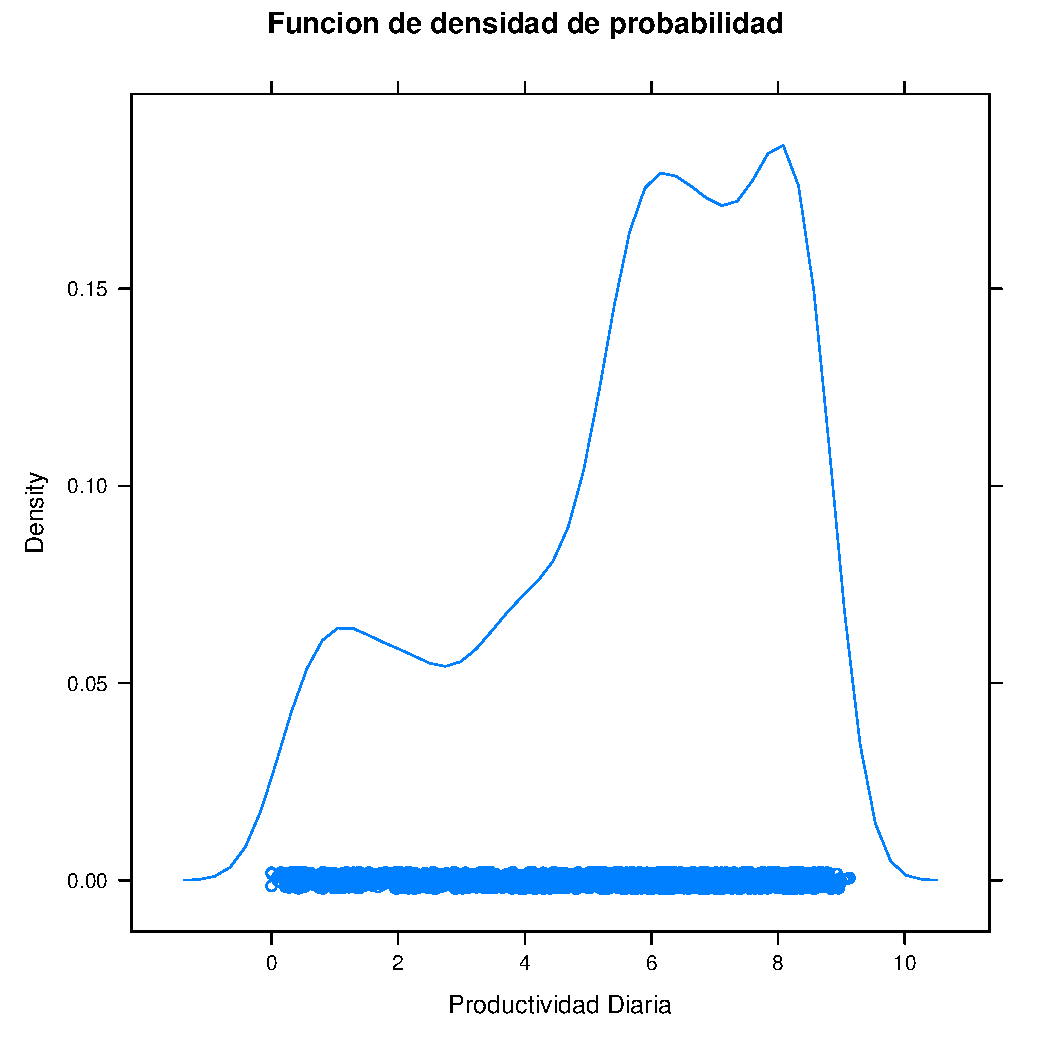
\includegraphics[width=.9\linewidth]{../figs/FuncionDensidadProbabilidad.pdf}
\end{center}
\end{frame}

\begin{frame}[label={sec:org04877b0}]{Histograma}
\begin{center}
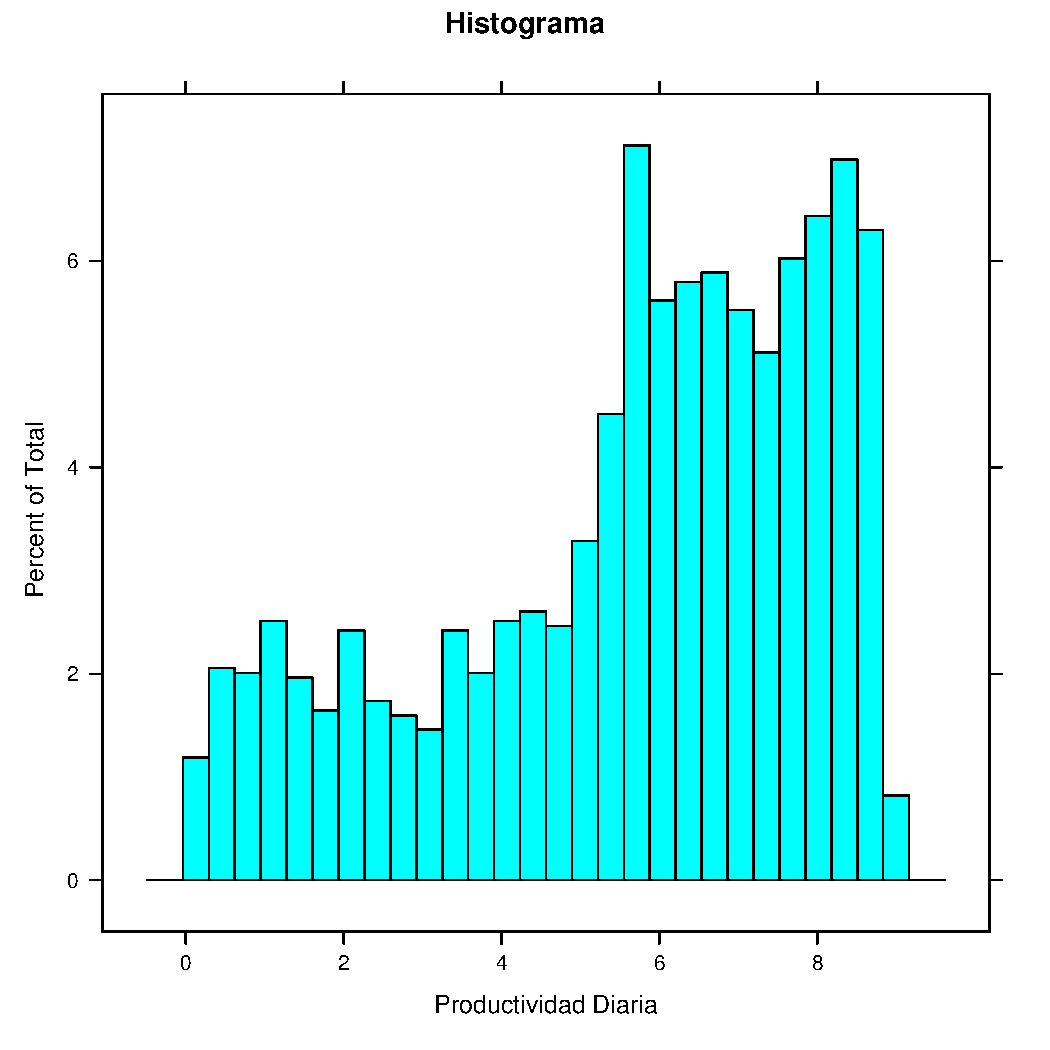
\includegraphics[width=.9\linewidth]{../figs/Histograma.pdf}
\end{center}
\end{frame}



\begin{frame}[label={sec:orge693f29}]{Media, varianza y desviación estándar}
\begin{itemize}
\item La \alert{media} de una variable aleatoria es el \alert{centro de masas} de su función densidad de probabilidad:
\end{itemize}

\[
\mu_{X}=\int_{-\infty}^{\infty}x\cdot f(x)dx
\]

\begin{itemize}
\item La \alert{varianza} de una variable aleatoria es la \alert{media del cuadrado de las desviaciones} respecto a la media:
\end{itemize}

\[
\sigma_{X}^{2}=\int_{-\infty}^{\infty}(x-\mu_{X})^{2}\cdot f(x)dx
\]

\begin{itemize}
\item La \alert{desviación estándar} es la raiz cuadrada de la varianza: \(\sigma_{X}=\sqrt{\sigma_{X}^2}\)
\end{itemize}
\end{frame}



\begin{frame}[label={sec:org3d2b6cf}]{Combinación lineal de variables aleatorias}
\begin{itemize}
\item La \alert{media de la suma} de varias variables aleatorias \alert{independientes} es
la suma de las medias:
\end{itemize}
\[
\mu_{X_{1}+...+X_{n}}=\mu_{X_{1}}+...+\mu_{X_{n}}
\]

\begin{itemize}
\item La \alert{varianza de la \emph{suma o resta}} de varias variables aleatorias
\alert{independientes} es la \alert{suma} de las varianzas:
\end{itemize}

\[
\sigma_{X_{1}\pm...\pm X_{n}}^{2}=\sigma_{X_{1}}^{2}+...+\sigma_{X_{n}}^{2}
\]
\end{frame}



\begin{frame}[label={sec:org2520a31}]{Media y varianza de la media muestral}
\begin{itemize}
\item Una \alert{muestra de una población} es un conjunto de variables
aleatorias independientes (\(X_{1}...X_{n}\)).

\item Si se toma una muestra de una población cuya media es \(\mu\) y su
varianza es \(\sigma^{2}\), entonces la media de la muestra es otra
variable aleatoria (que es una suma de variables aleatorias)
\end{itemize}

\[
\overline{X}=\frac{1}{n}\sum_{n}X_{i}
\]
\end{frame}



\begin{frame}[label={sec:orgc5e8b34}]{Media y varianza de la media muestral}
\begin{itemize}
\item Por tanto, la \alert{media de la media muestral} es la media de población:
\end{itemize}
\[
\overline{X}=\frac{1}{n}\sum_{n}X_{i} = \mu
\]

\begin{itemize}
\item La \alert{varianza de la media muestral} es la suma de las varianzas:
\end{itemize}

\[
\sigma_{\overline{X}}^{2}=\sigma_{\frac{1}{n}X_{1}}^{2}+...+\sigma_{\frac{1}{n}X_{n}}^{2}=\frac{\sigma^2}{N}
\]

\begin{block}{}
Por tanto, una forma de \alert{reducir la incertidumbre} es realizar la
\alert{medida en repetidas ocasiones}.
\end{block}
\end{frame}



\begin{frame}[label={sec:orgd221890}]{Mediana y cuartiles}
\begin{itemize}
\item La \alert{mediana} divide el conjunto de valores de la variable en \alert{dos
mitades} iguales (divide el area encerrada por la función densidad
de probabilidad en dos partes iguales).
\item Los \alert{cuartiles} dividen este area en \alert{cuatro} partes iguales.
\item El area encerrada entre cada par de cuartiles es igual al 25$\backslash$% del total.
\item La \alert{mediana} es el \alert{segundo cuartil}.
\item La \alert{distancia intercuartil} (definida entre los cuartiles 1 y 3) es
una \alert{medida de la dispersión} de la variable.
\end{itemize}
\end{frame}


\subsection{Gráficos}
\label{sec:org274bcf7}


\begin{frame}[label={sec:orgbd4e071}]{Función de Densidad de Probabilidad}
\begin{center}
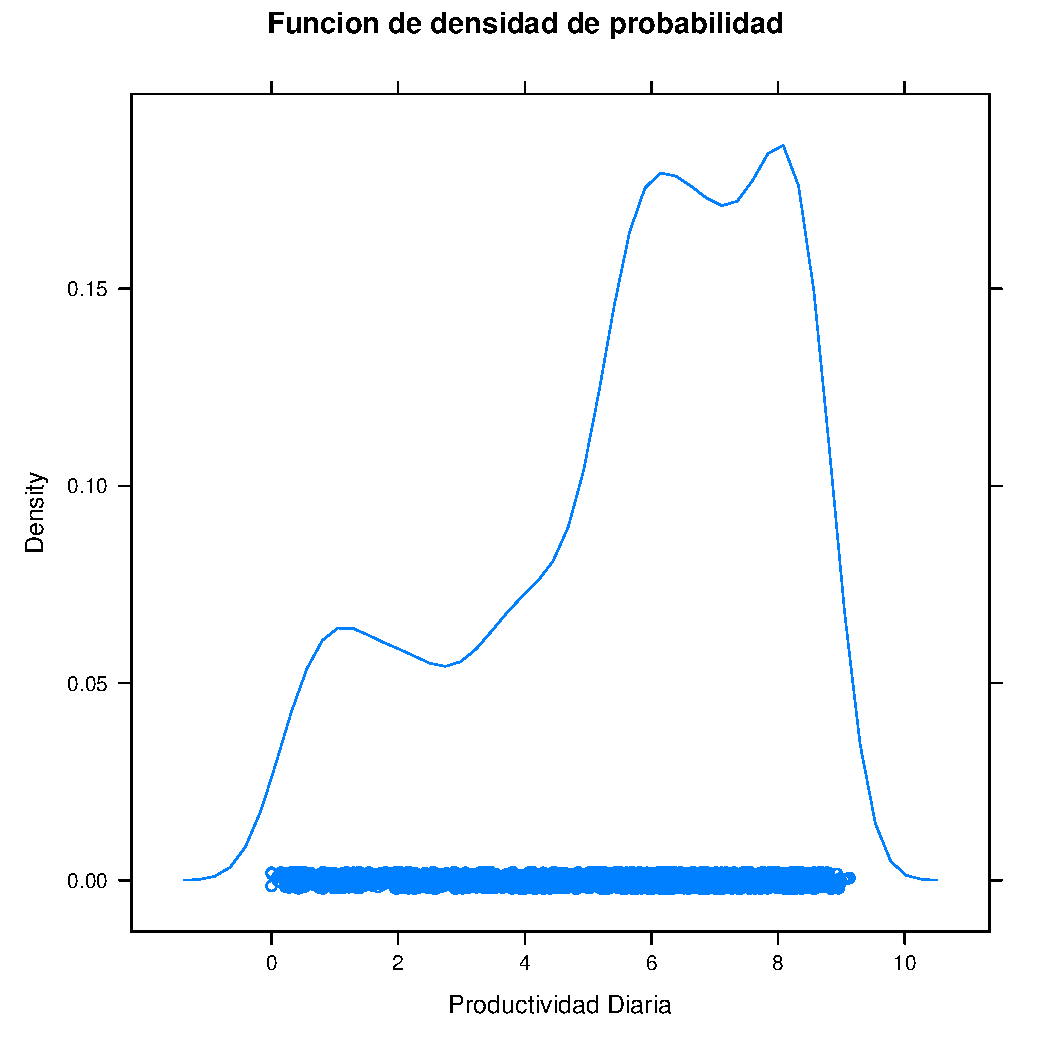
\includegraphics[width=.9\linewidth]{../figs/FuncionDensidadProbabilidad.pdf}
\end{center}
\end{frame}

\begin{frame}[label={sec:org63dedfb}]{Histograma}
\begin{center}
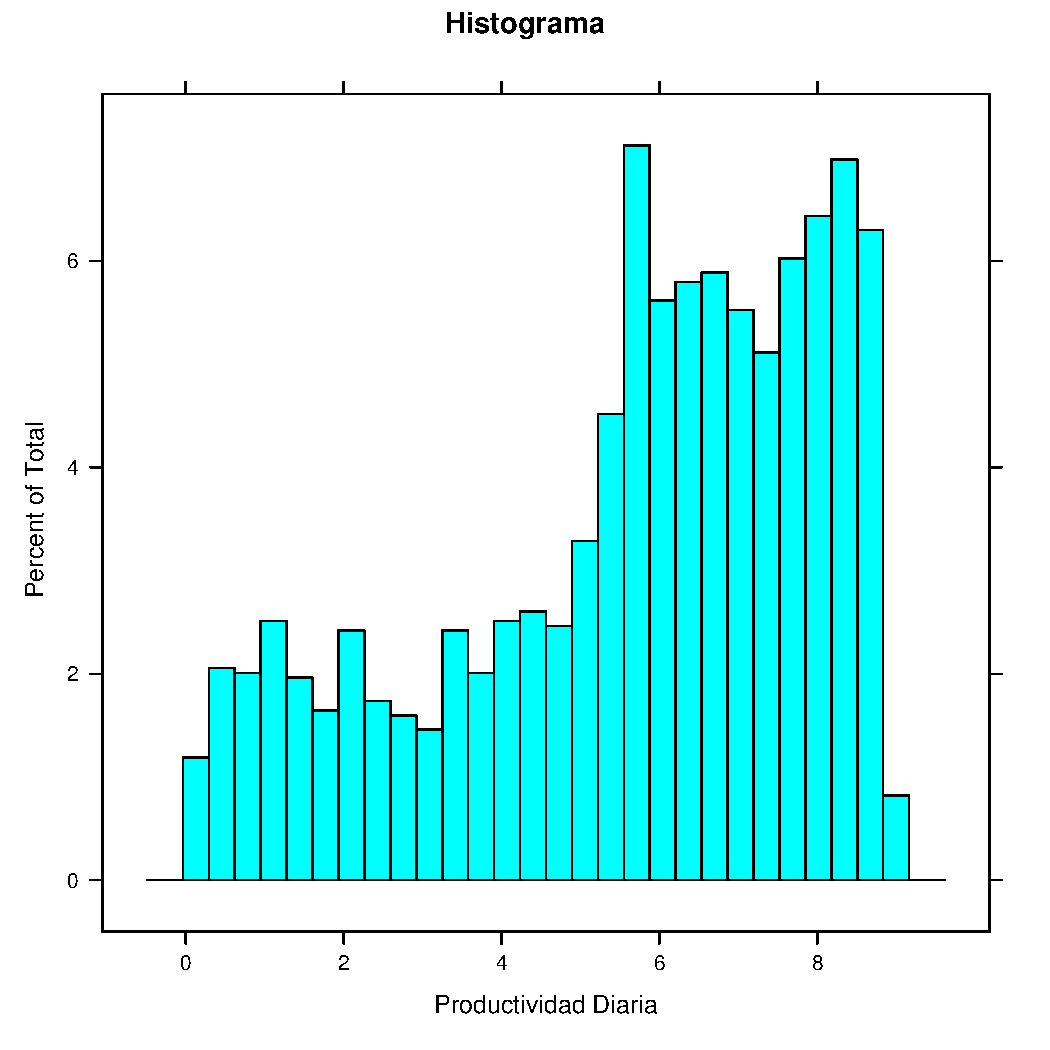
\includegraphics[width=.9\linewidth]{../figs/Histograma.pdf}
\end{center}
\end{frame}


\begin{frame}[label={sec:org9f2c462}]{Gráficos boxplot}
\begin{center}
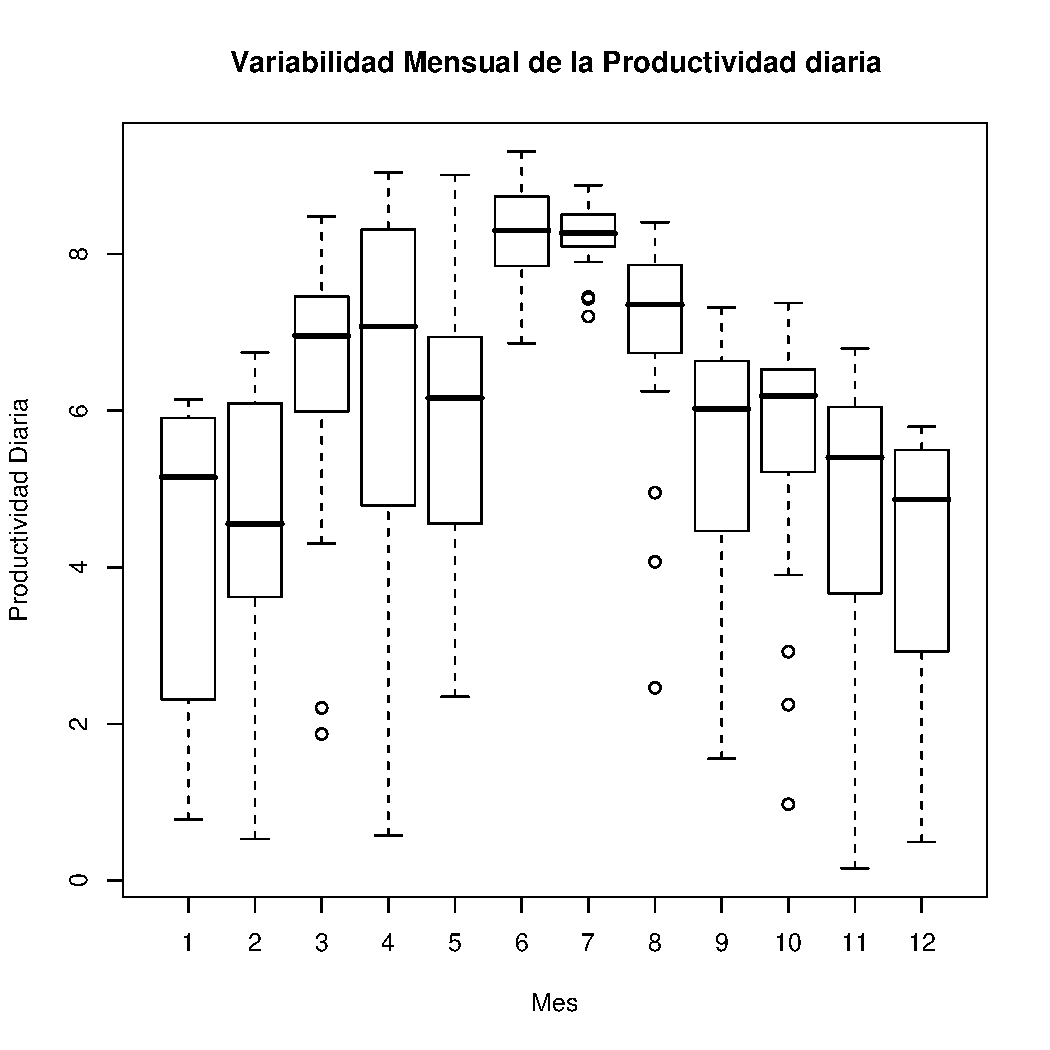
\includegraphics[width=.9\linewidth]{../figs/GraficoBoxplot.pdf}
\end{center}
\end{frame}


\begin{frame}[label={sec:org4d5ee9e}]{Gráficos de dispersión}
\begin{center}
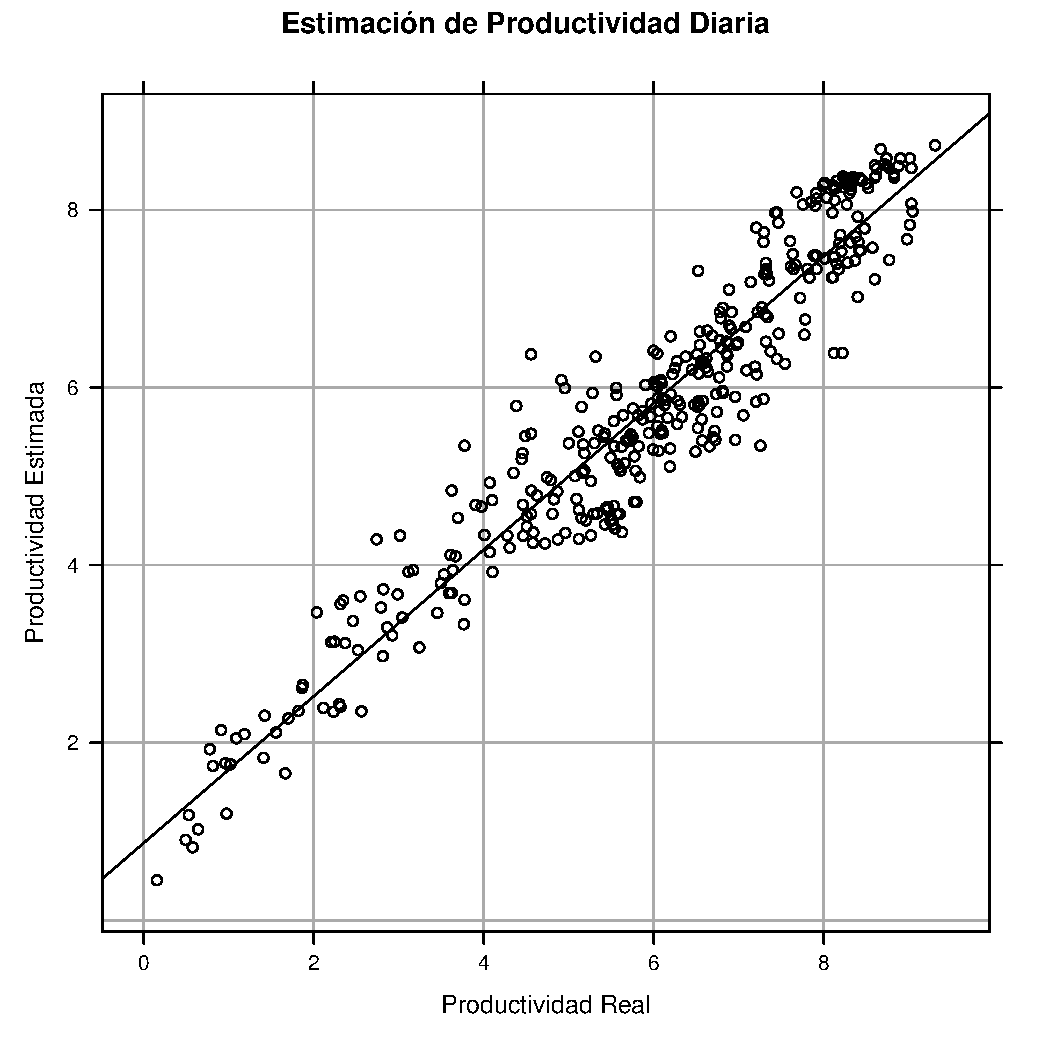
\includegraphics[width=.9\linewidth]{../figs/GraficoDispersion.pdf}
\end{center}
\end{frame}


\begin{frame}[label={sec:org768348c}]{Matrices de gráficos de dispersión}
\begin{center}
\includegraphics[height=0.9\textheight]{../figs/Splom.png}
\end{center}
\end{frame}

\subsection{Control de Calidad de Medidas}
\label{sec:orgac58e67}

\begin{frame}[label={sec:orgbc08c0d}]{Introducción}
\begin{block}{Las medidas recogidas por estaciones meteorológicas se deben filtrar para eliminar datos erroneos.}
\begin{itemize}
\item Límites Físicos
\item Tests de persistencia
\item Tests de rampas (irradiancia)
\item Tests de envolvente (medida de varias componentes)
\item Coherencia espacial
\item Coherencia estadística
\end{itemize}
\end{block}
\end{frame}



\begin{frame}[label={sec:orgf29bfcd}]{Límites físicos}
\begin{block}{Irradiación Diaria}
\begin{itemize}
\item La radiación global en el plano horizontal debe ser inferior a la extraterrestre (\(K_t \leq 1\))
\end{itemize}
\[
G_d(0) \leq B_od(0)
\]

\begin{itemize}
\item El índice de claridad debe ser superior a 0.03
\end{itemize}
\[
K_t = \frac{G_d(0)}{B_{od}(0)} \geq 0.03
\]

\begin{itemize}
\item La radiación global en el plano horizontal debe ser inferior a la de un modelo de cielo claro
\end{itemize}

\nocite{Younes.Claywell.ea2005, Estevez.Gavilan.ea2011, Geiger.Diabate.ea2002}
\end{block}
\end{frame}

\begin{frame}[label={sec:org506b4da}]{Límites físicos}
\begin{block}{Irradiancia (intradiaria)}
\begin{itemize}
\item El índice de claridad debe ser inferior a 1 cuando la altura solar es suficiente:
\end{itemize}
\[
k_t < 1  \text{ si } \gamma_s > 2\degree 
\]
\begin{itemize}
\item Límites inferiores para cielos cubiertos (baja transparencia atmosférica)
\end{itemize}
\[
k_t \geq 10^{-4} \cdot (\gamma_s - 10\degree)  \text{ si } \gamma_s > 10\degree
\]

\[
G \geq 0  \text{ si } \gamma_s \leq 10\degree
\]

\nocite{Journee.Bertrand2011}
\end{block}
\end{frame}

\begin{frame}[label={sec:org21a181c}]{Tests de persistencia}
\begin{block}{Variabilidad de irradiancia}
\begin{itemize}
\item La media y la desviación estándar se calculan con todas las muestras de un día completo.
\end{itemize}
\[
\frac{1}{8} \overline{k_t} \leq \sigma_{k_t} \leq 0.35
\]
\end{block}
\end{frame}

\begin{frame}[label={sec:org4010a60}]{Tests de rampas}
\begin{block}{Límites a las variaciones de la irradiancia entre instantes sucesivos}
\[
\left| k_t(t) - k_t(t-1)\right| < 0.75 \text{ si } \gamma_s(t) > 2\degree
\]
\end{block}
\end{frame}


\begin{frame}[label={sec:orgc46b751}]{Tests de envolvente}
\begin{itemize}
\item Sólo para estaciones con medida simultánea de global y directa/difusa.
\end{itemize}

\begin{center}
\includegraphics[width=.9\linewidth]{../figs/ConsistencyTest.png}
\end{center}

\nocite{Younes.Claywell.ea2005}
\end{frame}

\begin{frame}[label={sec:orge9b1799}]{Coherencia espacial}
\begin{itemize}
\item Las medidas de una estación se pueden comparar con las recogidas por estaciones cercanas.
\item Esta comprobación debe realizarse con \alert{datos agregados} (diarios) (la variabilidad espacial intradiaria puede ser alta)
\item Esta comprobación debe realizarse con estaciones que tienen \alert{clima y geografía similar}.
\end{itemize}

\nocite{Journee.Bertrand2011}
\end{frame}

\begin{frame}[label={sec:org3bc2677}]{Coherencia espacial}
\begin{block}{Pasos}
\begin{itemize}
\item Estimamos la irradiación en el lugar, \(x_0\), con la interpolación espacial de las estaciones cercanas, \(x_i\).
\begin{itemize}
\item Los pesos \(w_i\) son una función inversa de la distancia (IDW).
\end{itemize}
\end{itemize}
\[
\widehat{G}_d(x_0) = \frac{\sum_{i=1}^N w_i G_{d}(x_i)}{\sum_{i=1}^N w_i} 
\]
\begin{itemize}
\item Comparamos la irradiación estimada, \(\widehat{G}_d(x_0)\), con la medida en la estación, \(G_d(x_0)\).
\end{itemize}
\[
\left| \widehat{G}_d(x_0) - G_d(x_0) \right|
\]
\begin{itemize}
\item La diferencia absoluta debe estar por debajo de un límite (p.ej. 50\%)
\end{itemize}
\end{block}
\end{frame}



\begin{frame}[label={sec:orgfcc8332}]{Coherencia estadística}
\begin{block}{Una medida puede ser etiquetada como \emph{outlier} si es poco probable que pertenezca a la misma distribución que el conjunto.}
\end{block}
\begin{block}{\alert{Método de Chauvenet}}
Una medida es un \emph{outlier} si la probabilidad de obtener su desviación
respecto de la media es inferior al inverso de 2 veces el número de
elementos en el conjunto.

\begin{center}
\includegraphics[width=.9\linewidth]{../figs/chauvenet.png}
\end{center}
\end{block}
\end{frame}

\begin{frame}[label={sec:org671967c}]{Método de Chauvenet}
\begin{itemize}
\item Sean \(G_d(x_i)\) las medidas de radiación diaria del conjunto formado por N estaciones.
\end{itemize}

\pause

\begin{itemize}
\item Se calcula la media, \(\overline{G}_d\), la desviación estándar, \(\sigma_{G_d}\).
\end{itemize}

\pause

\begin{itemize}
\item Se calcula la distancia estadística de cada estación al conjunto:
\end{itemize}
\[
d_i = \frac{G_d(x_i) - \overline{G}_d}{\sigma_{G_d}}
\]

\pause

\begin{itemize}
\item En una distribución gaussiana se calcula la distancia estadística
equivalente a la probabilidad límite, \(1/2N\), teniendo en cuenta
las dos colas.
\begin{itemize}
\item Por ejemplo, para un conjunto de 10 estaciones cada cola es
\(1/40 = 0.025\), el límite es \(\left| d_{max} \right| = 1.96\).
\end{itemize}
\end{itemize}
\pause

\begin{itemize}
\item Aquellas observaciones que superan la distancia son marcadas como outliers.
\end{itemize}

\nocite{Perpinan2009}
\end{frame}

\begin{frame}[label={sec:orgeba12b6}]{Método de Chauvenet}
\[
d_i = \frac{G_d(x_i) - \overline{G}_d}{\sigma_{G_d}}
\]

\[
\left| d_i \right| > \left| d_{max} \right|
\]

\begin{center}
\begin{center}
\includegraphics[width=.9\linewidth]{../figs/chauvenet.png}
\end{center}
\end{center}

\begin{block}{Método de Pierce: más robusto y flexible \nocite{Ross2003}}
\end{block}
\end{frame}

\subsection{Control de Calidad de Modelos}
\label{sec:org385acfc}

\begin{frame}[label={sec:orgc2d4a93}]{Desviación entre modelo y observación}
\begin{itemize}
\item Sea \(O\) el conjunto de observaciones (medidas) de una variable aleatoria.
\end{itemize}

\[
\mathbf{O} = \left\{ o_1 \dots o_n \right\}
\]
\begin{itemize}
\item Sea \(M\) el conjunto de resultados de un modelo que aproxima el comportamiento de la variable medida.
\end{itemize}

\[
\mathbf{M} = \left\{ m_1 \dots m_n  \right\}
\]

\begin{itemize}
\item La desviación entre modelo y observación es:
\end{itemize}

\[
\mathbf{D} = \mathbf{M} - \mathbf{O} =  \left\{ (m_1 - o_1) \dots (m_n - o_n)  \right\} = \left\{ d_1 \dots d_n  \right\}
\]
\end{frame}

\begin{frame}[label={sec:orgf5d3d38}]{Estimadores frecuentes: MBD y RMSD}
\begin{itemize}
\item Mean Bias Difference (MBD), diferencia media (indica si el modelo sobreestima o subestima):
\end{itemize}
\[
MBE = \overline{\mathbf{D}} = \overline{\mathbf{M}} - \overline{\mathbf{O}} = \frac{1}{n} \sum_{i=1}^n (m_i - o_i)
\]
\pause
\begin{itemize}
\item Root Mean Square Error (RMSD), diferencia cuadrático media:
\end{itemize}
\[
RMSD = \left(\frac{1}{n} \sum_{i=1}^n d_i^2 \right)^{1/2} =  \left( \frac{1}{n} \sum_{i=1}^n (m_i - o_i)^2  \right)^{1/2}
\]
\end{frame}

\begin{frame}[label={sec:org2d5a669}]{Estimadores frecuentes: MBE y RMSD}
\begin{itemize}
\item Varianza de la diferencia (unbiased RMSD):
\end{itemize}
\[
\sigma^2_{\mathbf{D}} = \frac{1}{n} \sum_{i=1}^n (d_i - \overline{\mathbf{D}})^2
\]
\pause

\begin{itemize}
\item El RMSD agrega información del promedio y la varianza de la
diferencia:
\end{itemize}
\[
RMSD^2= \sigma^2_{\mathbf{D}} + \overline{\mathbf{D}}^2
\]
\end{frame}

\begin{frame}[label={sec:orgc1a5b3f}]{Otros estimadores: MAD}
\begin{itemize}
\item Mean Absolute Deviation (MAD):
\end{itemize}

\[
MAD = \frac{1}{n} \sum_{i=1}^n \left|d_i\right| =  \frac{1}{n} \sum_{i=1}^n \left|m_i - o_i\right|
\]
\begin{itemize}
\item El RMSD no es robusto (un error puntual puede distorsionar el estimador) y depende del número de muestras:
\end{itemize}
\[
MAD \leq RMSD \leq n^{1/2} MAD
\]

\nocite{Willmott.Matsuura.ea2009, Willmott.Matsuura2005a}
\end{frame}

\begin{frame}[label={sec:org1fbcdb1}]{Otros estimadores: t y d}
\begin{itemize}
\item t de Student (valores pequeños indican buen comportamiento del modelo)
\begin{itemize}
\item Permite añadir intervalos de confianza a las diferencias entre
modelo y observación
\end{itemize}
\end{itemize}

\[
t = \left ( \frac{(n-1) MBD^2}{RMSD^2 - MBD^2} \right)^{1/2}
\]

\nocite{Stone1993}

\pause 

\begin{itemize}
\item \(d_1\): Índice de concordancia de Willmott.
\begin{itemize}
\item Limitado entre 0 (ausencia de concordancia) y 1 (concordancia total).
\item Robusto frente a \emph{outliers}.
\end{itemize}
\end{itemize}
\[
d_1 = 1 - \frac{\sum_{i=1}^n \left| m_i - o_i \right|}{\sum_{i=1}^n \left(
  \left| m_i - \overline{\mathbf{O}}\right| + \left| o_i -
    \overline{\mathbf{O}} \right| \right)}
\]

\nocite{Willmott.Robeson.ea2012}
\end{frame}

\begin{frame}[label={sec:org3af66bf}]{Correlación}
El coeficiente de correlación entre dos conjuntos de datos es una
medida numérica de la relación \alert{lineal} entre los dos conjuntos (si la
relación no es lineal, este coeficiente no sirve):

\[
r = \frac{1}{n-1} \cdot \sum_{i=1}^{n} \left( \frac{o_{i}-\overline{\mathbf{O}}}{\sigma_{\mathbf{O}}}\right) \cdot \left(\frac{m_{i}-\overline{\mathbf{M}}}{\sigma_{\mathbf{M}}}\right)
\]
\end{frame}

\begin{frame}[label={sec:org6735254}]{Diagramas de Taylor}
\begin{itemize}
\item Desarrollando \(\sigma^2_{\mathbf{D}}\) y teniendo en cuenta la definición de \(r\):
\end{itemize}

  \[
  \sigma^2_{\mathbf{D}} = \sigma^2_{\mathbf{O}}  + \sigma^2_{\mathbf{M}}
- 2 \cdot \sigma_{\mathbf{O}} \cdot \sigma_{\mathbf{M}} \cdot r
  \]
\begin{itemize}
\item Esta relación es semejante a la ley de los cosenos (\(c\), \(a\), \(b\) son lados de un triángulo y \(\phi\) es el ángulo opuesto al lado \(c\)):
\end{itemize}

\[
c^2 = a^2 + b^2 - 2 \cdot a \cdot b \cos\phi
\]
\nocite{Taylor2000}
\end{frame}

\begin{frame}[label={sec:org3a8f334}]{Diagramas de Taylor}
\[
\sigma^2_{\mathbf{D}} = \sigma^2_{\mathbf{O}}  + \sigma^2_{\mathbf{M}}
- 2 \cdot \sigma_{\mathbf{O}} \cdot \sigma_{\mathbf{M}} \cdot r 
\]

\begin{center}
\begin{center}
\includegraphics[width=.9\linewidth]{../figs/cosenosDiagramaTaylor.png}
\end{center}
\end{center}
\end{frame}

\begin{frame}[label={sec:org157802d}]{Diagramas de Taylor}
\begin{itemize}
\item \(\sigma^2_{\mathbf{D}}\): Distancia al origen
\item \(\sigma^2_{\mathbf{O}}\): Eje horizontal
\item \(\sigma^2_{\mathbf{M}}\): Eje vertical
\item \(r\): acimut
\end{itemize}
\begin{center}
\begin{center}
\includegraphics[height=0.6\textheight]{../figs/TaylorDiagrama.png}
\end{center}
\end{center}
\end{frame}


\begin{frame}[label={sec:org42ec4e3}]{Target Diagram}
\begin{itemize}
\item Emplea la relación entre \(RMSD\), \(\sigma^2_{\mathbf{D}}\), y \(\overline{\mathbf{D}}\), normalizadas con \(\sigma_{\mathbf{O}}\):
\end{itemize}
\[
RMSD' = RMSD / \sigma_{\mathbf{O}}
\]

\[
  \sigma'_{\mathbf{D}} = \sigma_{\mathbf{D}} / \sigma_{\mathbf{O}} 
\]

\[
\overline{\mathbf{D}}' = \overline{\mathbf{D}} / \sigma_{\mathbf{O}}
\]

\[
RMSD'^2= \sigma'^2_{\mathbf{D}} + \overline{\mathbf{D}}'^2
\]

\[
sign_{\sigma} =  sign(\sigma_{\mathbf{M}} - \sigma_{\mathbf{O}} )
\]

\begin{itemize}
\item Incorporan el signo de la diferencia entre desviaciones estándar de modelo y observación:
\end{itemize}

\nocite{Jolliff.Kindle.ea2009}
\end{frame}

\begin{frame}[label={sec:org2a6fccb}]{Target Diagram}
\begin{itemize}
\item \(\sigma'_{\mathbf{D}}\) (con signo): Eje horizontal
\item \(\overline{\mathbf{D}}'\): Eje vertical
\item \(RMSD'^2\): Distancia al origen
\end{itemize}

\begin{center}
\begin{center}
\includegraphics[height=0.7\textheight]{../figs/TargetDiagram.pdf}
\end{center}
\end{center}
\end{frame}
\end{document}